\chapter{Diseño\label{sec:Diseno}}

Este proyecto consiste en una \textbf{ampliación y cambio de enfoque} de otro proyecto llevado a cabo de manera simultánea por una alumna de la Universidad Politécnica de Madrid llamada Nerea Urrestarazu que, a su vez, se basa en el Kit de demostración de rendimiento del ADS1299 proporcionado por Texas Instrument.

\begin{figure} [h]
    \centering
    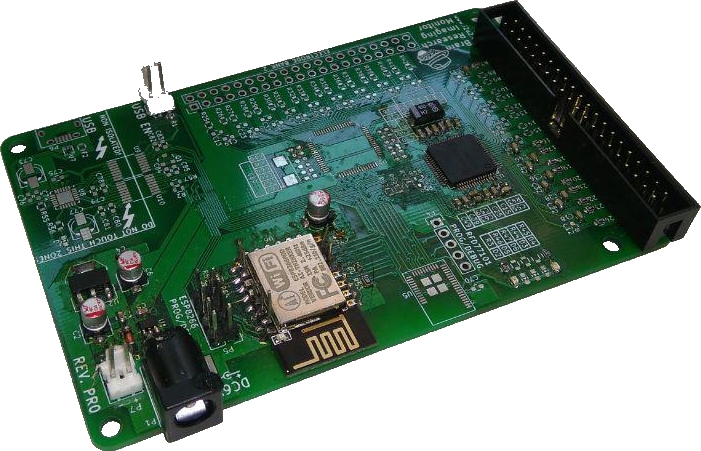
\includegraphics[width=7cm]{Placa_Nerea}
    \caption{Placa final del proyecto base}
    \label{fig:Placa_base}
\end{figure}

\section{Diseño base\label{sec:Diseno_base_N}}

El \textbf{proyecto original} consiste en el \textbf{diseño y desarrollo} de una \textbf{placa de adquisición de \acrshort{EEG}} haciendo uso de los integrados ADS1299 junto con un sistema de transmisión hacia el ordenador tanto inalámbricamente como a través de USB. La figura \ref{fig:Diseno_base} muestra las partes que componen dicho diseño.

\begin{figure} [h]
    \centering
    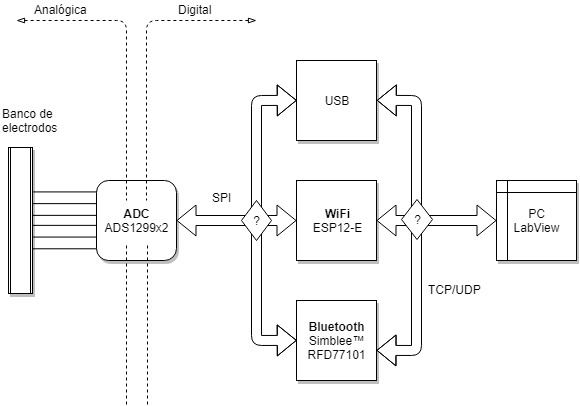
\includegraphics[width=12cm]{Esquema_diseno_base}
    \caption{Esquema del proyecto base}
    \label{fig:Diseno_base}
\end{figure}

\subsection{Adquisición de datos\label{sec:Adquisicion_N}}

La parte encargada de la \textbf{adquisición} está compuesta por un par de \textbf{bancos de electrodos} dispuestos en los laterales de la placa seguidos por un filtro paso-bajo con frecuencia de corte de 6.79kHz, encargado de eliminar las componentes de frecuencias muy altas, no deseadas en el estudio de un \acrshort{EEG}. A continuación se encuentran conectados a sus respectivos bancos los \textbf{\acrshort{ADC} ADS1299}. 
\\Estos convertidores son capaces de adquirir información de forma independiente o en modo ``\textit{Daisy Chain}'' y \textbf{transmitirla a través de \acrshort{SPI}} hacia otros dispositivos cuya misión será gestionarla.

\begin{figure} [h]
    \centering
    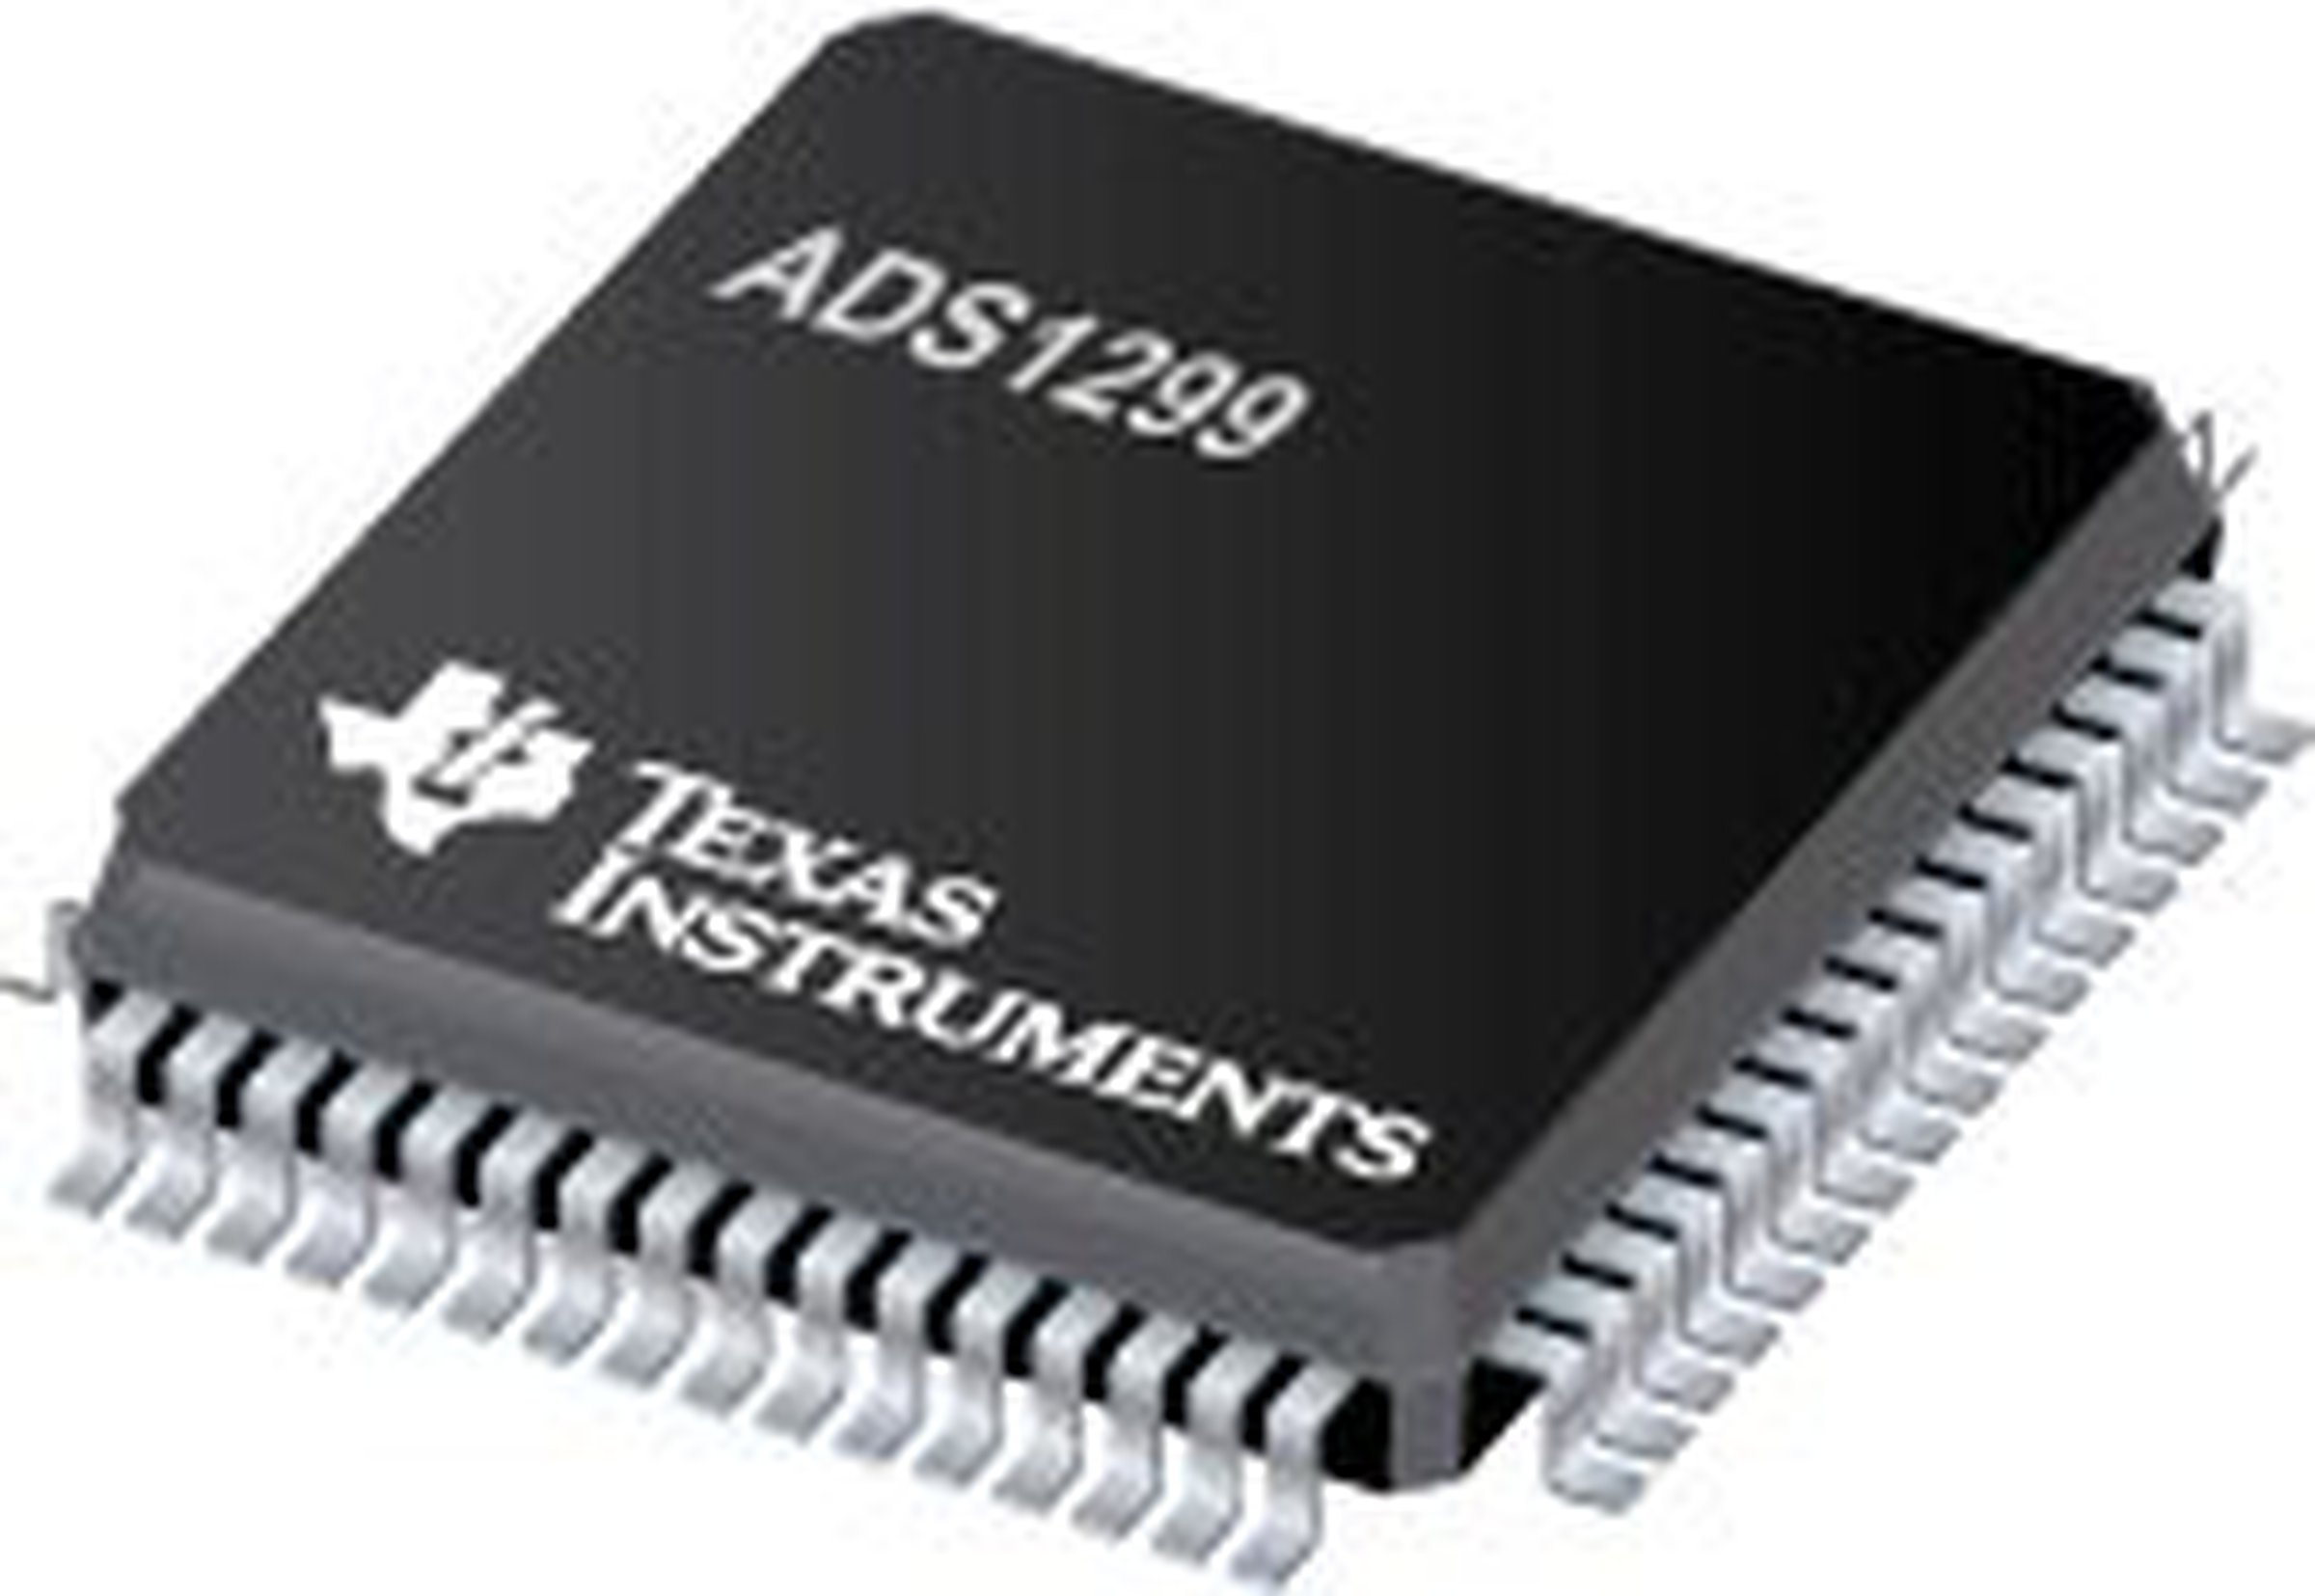
\includegraphics[width=6cm]{ADS1299}
    \caption{Convertidor Analógico-Digital ADS1299}
    \label{fig:ADS1299}
\end{figure}

El \acrshort{SPI} presente en el convertidor permite leer todos los registros del ADS y escribir la gran mayoría. Aunque normalmente se leen los relacionados con los datos convertidos, también es posible saber el estado de los \acrshort{GPIO} o el identificador único del dispositivo leyendo su registro asociado.

La \textbf{configuración} del ADS se realiza mediante la \textbf{escritura de ciertos registros}, cada uno asociado a un parámetro específico. La tabla \ref{tab:Conf_Reg_ADS} muestra los registros disponibles, tanto de lectura como de configuración, una descripción básica y la dirección de memoria asociada a los mismos.

\begin{table} [h]
    \centering
    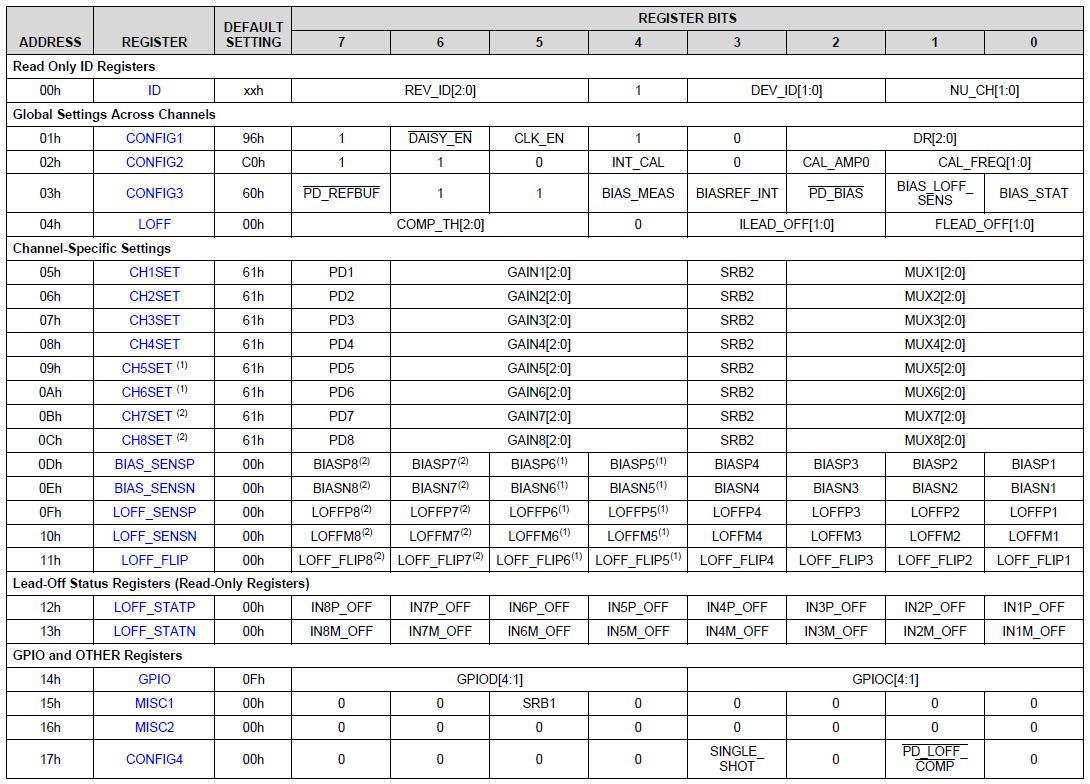
\includegraphics[width=\textwidth]{Tabla_registros_ADS}
    \caption{Tabla de registros de la familia ADS \cite{Datasheet_ADS}}
    \label{tab:Conf_Reg_ADS}
\end{table}

Una descripción más detallada de cada uno de los bits de cada registro se puede encontrar en el \textit{datasheet} del componente \cite{Datasheet_ADS}.

Como se puede ver en la tabla \ref{tab:Conf_Reg_ADS}, los convertidores cuentan con una gran cantidad de opciones de configuración. Para el desarrollo de este proyecto \textbf{se ha implementado un sistema de configuración que permite la lectura y escritura de todos los registros}.

\subsection{Transmisión de datos\label{sec:Transmisión_N}}

Tras completar el proceso de adquisición de datos resulta necesario transmitir dicha información hacia un dispositivo capaz de procesarla. Para ello la placa original contaba con dos alternativas. La primera consiste en, mediante \textbf{\acrshort{USB}} y acopladores aislantes, transmitir la información a un ordenador. 
\\La segunda hace uso de dos tecnologías inalámbricas distintas que funcionan de forma excluyente y son seleccionables con un \textit{jumper}: \textbf{WiFi} o \textbf{Bluetooth}.

\subsubsection{WiFi\label{sec:WiFi_N}}

Para la transmisión de datos a través de \textbf{WiFi} se seleccionó el \textbf{módulo ESP12-E}, basado en el \acrshort{SoC} ESP2866, también conocido nodemcu.
\\Este cuenta con un microcontrolador (\acrshort{MCU}) embebido de 32 bits (Tensilica L106) con una memoria \acrshort{RAM} de 36kB y una velocidad de reloj de la \acrshort{CPU} de hasta 80MHz, proporcionando suficiente potencia para las tareas básicas.

Así mismo se incluye montado en el mismo paquete una memoria flash de 4MB en la que almacenar el código de los programas que se ejecutarán y una antena embebida, dotando al módulo de conectividad en la banda de 2.4GHz.

\begin{figure} [h]
    \centering
    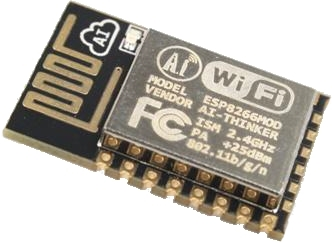
\includegraphics[width=6cm]{ESP8266}
    \caption{ESP8266}
    \label{fig:ESP8266}
\end{figure}

A efectos de diseño es muy importante saber cuales serán las entradas/salidas del dispositivo así como los \textbf{pines dedicados para su programación}. La figura \ref{fig:ESP8266_pinout} muestra un resumen de todas las funciones de cada uno de los pines. Como se puede observar, el \acrshort{SPI} hace uso de los pines 5, 6, 7 y 16. Por otro lado el \acrshort{UART}, necesario para la programación del micro hace uso de los pines 16 y 17. Dichos pines deberán \textbf{reservarse} posteriormente en la fase de diseño de la \acrshort{PCB}.

El dispositivo tiene tres modos de arranque dependiendo del sitio desde el que cargue el código y la selección de uno u otro modo viene determinada por los pines MTDO, GPIO0 y GPIO2. \\La tabla \ref{tab:ESP_Boot_Modes} los distintos modos de arranque y el estado en el que deben estar de los pines para iniciar en dicho modo.
\begin{table} [h]
 	\centering
	\begin{tabular}{|c|c|c|c|c|}
		\hline 
		MTDO & GPIO0 & GPIO2 & Modo & Descripción \\ 
		\hline 
		L & L & H & UART & Descarga el código desde UART \\ 
		\hline 
		L & H & H & Flash & Carga desde memoria Flash a través de SPI \\ 
		\hline 
		H & x & x & SDIO & Carga desde una tarjeta SD \\ 
		\hline 
	\end{tabular} 
	\caption{Modos de arranque del ESP12-E \cite{ESP_Boot_mode}}
    \label{tab:ESP_Boot_Modes}
\end{table}	

\clearpage

\begin{figure} [h]
    \centering
    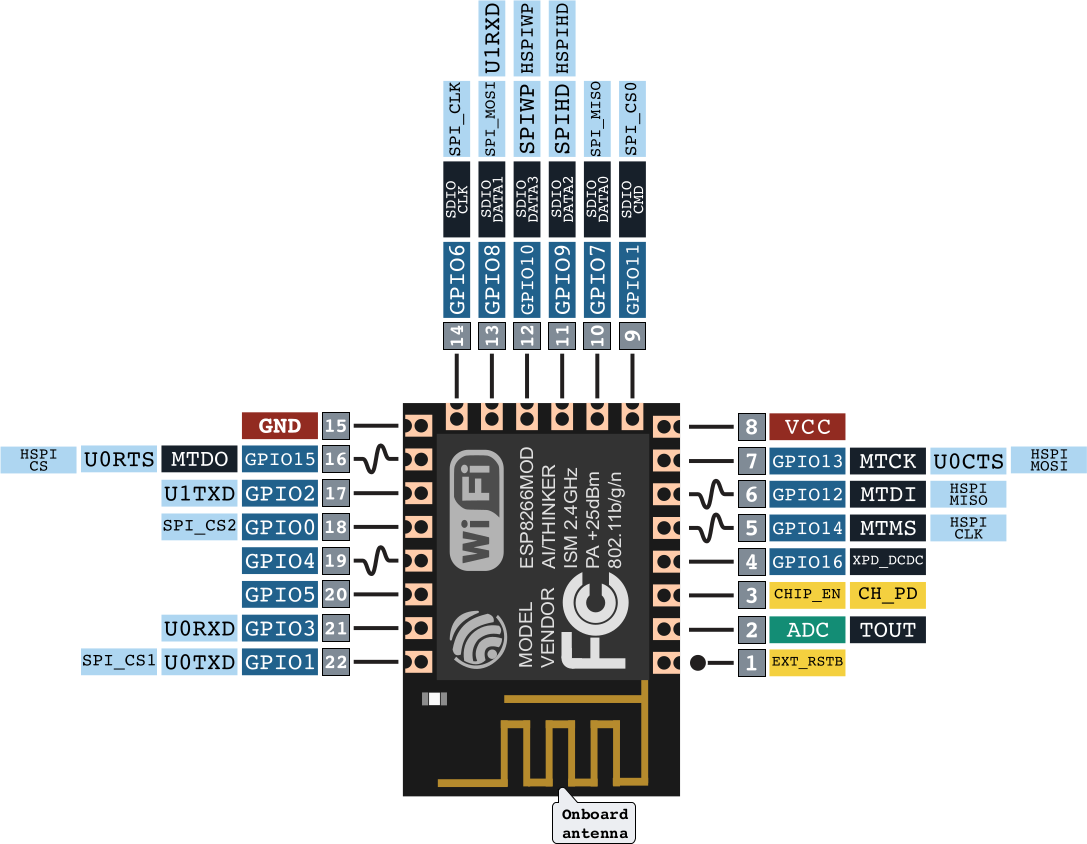
\includegraphics[width=15cm]{esp8266-esp12e-pinout}
    \caption{Resumen de todas las Entradas/Salidas del ESP12-E \cite{ESP_Pinout}}
    \label{fig:ESP8266_pinout}
\end{figure}

\subsubsection{Bluetooth\label{sec:Bluetooth_N}}

Para la transmisión de datos a través de \textbf{Bluetooth} se seleccionó el módulo Simblee™ RFD77101 ya que al igual que el módulo WiFi, cuenta con interfaces de \textbf{comunicación a través de \acrshort{SPI}} para conectarse con el \acrshort{ADC} (pines 21, 22, 31 y 32) y de \acrshort{UART} para su programación posterior programación (pines 23 y 24).

\begin{figure} [H]
    \centering
    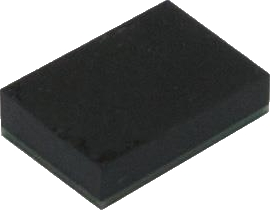
\includegraphics[width=5cm]{BT}
    \caption{Simblee™ RFD77101 \cite{Datasheet_BT}}
    \label{fig:BT}
\end{figure}

El módulo presenta un ARM Cortex-M0 como \acrshort{CPU} con 128KB de memoria Flash, 24KB de \acrshort{RAM} y una frecuencia de reloj de 16MHz. 

Todos los dispositivos de transmisión inalámbrica anteriormente mencionados permiten su \textbf{programación utilizando el \acrshort{IDE} de Arduino} lo cual facilita sensiblemente el proceso de desarrollo y prototipado teniendo la ventaja adicional de que es Software Libre.


\subsubsection{USB\label{sec:USB_N}}


Como este proyecto tiene como objetivo independizar el sistema lo máximo posible del ordenador se ha optado por \textbf{desestimar} el sistema de transmisión por \acrshort{USB} conservando solamente la interfaz inalámbrica. 

\section{Diseño final\label{sec:Diseño_final}}
          
Llegados a este punto se han analizado las características más importantes de cada uno de los elementos presentes en el sistema original, siendo los más importantes las distintas interfaces de comunicación y los pines de programación.
\\Con esta información ya es posible independizar cada uno de esos elementos y crear un \textbf{nuevo diseño que cumpla con las especificaciones de este proyecto}.

\begin{figure} [h]
    \centering
    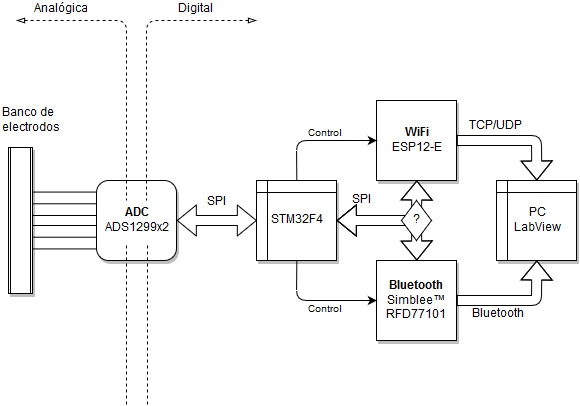
\includegraphics[width=13cm]{Esquema_proyecto_Javier}
    \caption{Esquema del proyecto final}
    \label{fig:Esquema_proyecto_Javier}
\end{figure}

\clearpage

El nuevo sistema estará compuesto por \textbf{tres partes}:
\begin{itemize}
\item En primer lugar etapa de \textbf{adquisición} compuesta de un \textbf{banco de electrodos} con sus correspondientes filtros analógicos y \textbf{dos \acrshort{ADC}}. 
\item Posteriormente un \textbf{microcontrolador} se encargará de realizar el \textbf{procesado} de la señal y la \textbf{gestión} de los distintos elementos.
\item Por último la transmisión de datos se realizará de forma \textbf{inalámbrica} a un ordenador u otro dispositivo mediante \textbf{Bluetooth o WiFi}.
\end{itemize}

Como se puede observar en la figura \ref{fig:Esquema_proyecto_Javier}, el ordenador sigue estando presente en el sistema pero en esta ocasión su función se limita a mostrar la información siendo fácilmente sustituible en un futuro por un dispositivo menos potente y barato. Al utilizar un microcontrolador en la propia placa de adquisición se consigue aumentar la independencia del sistema y se dota de unas características muy interesantes, tanto de procesado de señal como de almacenaje de la misma o gestión del consumo.

\subsection{Selección del microcontrolador\label{sec:Sel_micro}}

\textbf{El microcontrolador es el núcleo del sistema}. Para poder interactuar con todos los elementos anteriormente descritos deberá contar con las siguientes características:
\begin{itemize}
\item Bajo precio.
\item Bajo consumo.
\item Capacidad procesado de señal.
\item Para poder utilizar el máximo de la velocidad de adquisición de los ADS (16k\acrshort{SPS}) y evitar cuellos de botella, deberá contar con un Bus SPI de al menos 5.85Mb/s dedicados para la transmisión y la misma cantidad para recepción o dos buses.
\[Tasa\ de\ transferencia = 16k\ Muestras/s * 8\ canales * 24bits * 2\ ADS = 5.85Mb/s\]

\end{itemize}

Hay una gran cantidad de microcontroladores en el mercado que podrían utilizarse para este proyecto pero, de entre todos los disponibles, aquellos con arquitectura \textbf{ARM} son los que mejor se adaptan a las especificaciones. Concretamente los más adecuados son aquellos englobados en la familia \textbf{Cortex M4} ya que están especialmente diseñados con \acrshort{DSP} integrado para conseguir un \textbf{rendimiento máximo minimizando el consumo}.

\begin{figure}[H]
  \centering
  \begin{subfigure}[b]{0.49\textwidth}
   	\centering
    
\includegraphics [height=1.5cm]{Texas_Instument}
    \caption{Logo de Texas Instument \cite{Texas_Instrument}}
    \label{fig:Logo_TI}
  \end{subfigure}
  \hfill
  \begin{subfigure}[b]{0.49\textwidth}
  	\centering
    
\includegraphics[height=1.5cm]{STMicroelectronics}
    \caption{Logo de STMicroelectronics\cite{STMicroelectronic}}
    \label{fig:Logo_STM}
  \end{subfigure}
  \caption{Principales fabricantes contemplados}
\end{figure}

La tabla \ref{tab:Comparativa_MCU} muestra varios dispositivos de esa familia vendidos por Texas Instrument o STMicroelectronics y un resumen de sus características principales.
\begin{table} [h]
	\centering
	\begin{tabular}{|c|c|c|c|c|}
\hline 
 &\multicolumn{2}{c|}{\textbf{Texas Instruments}}& \multicolumn{2}{c|}{\textbf{STMicroelectronics}} \\ 
\hline 
 & TM4C123GH6PM & TM4C1294NCPDT & STM32F405& STM32F469  \\ 
\hline 
\acrshort{FCPU} [MHz] & 80 & 120 & 168 & 180 \\ 
\hline 
Flash [kB] & 256 & 1024 & 1024 & 2048 \\ 
\hline 
\acrshort{RAM} [kB] & 32 & 256 & 192 & 384 \\ 
\hline 
\acrshort{SPI} & x4 & x4 & x2 + 1 & x6 \\ 
\hline 
Precio [€] & 8,72 & 12,74 & 9,24 & 13,48 \\ 
\hline 
	\end{tabular} 
	\caption{Comparativa entre distintos MCUs}
	\label{tab:Comparativa_MCU}
\end{table}

Todos los dispositivos anteriormente contemplados tienen \acrshort{DSP} integrados así como una Unidad de Punto Flotante (\acrshort{FPU}) que permite realizar \textbf{operaciones matemáticas avanzadas} de forma óptima.

Entre los dispositivos anteriores, los pertenecientes a la familia \textbf{STM} presentan mejor relación coste/prestaciones, pero el verdadero factor diferenciador son las herramientas dispuestas para la comunidad por parte del fabricante.
\\En la página web se pueden encontrar distintas \textbf{aplicaciones} y \textbf{documentación} que facilitan sensiblemente el proceso de desarrollo para esta plataforma. 

Finalmente se seleccionó el \textbf{\acrshort{MCU} STM32F405} en el formato \textbf{\acrshort{LQFP64}} ya que sus características se ajustan perfectamente a las especificaciones, manteniendo unas muy buenas prestaciones y un precio bastante bajo. Todo esto con el valor añadido de que ya se contaba con la placa de desarrollo \textbf{STM32F4 Discovery} lo cual permitió comenzar con el aprendizaje y estudio del entorno sin la necesidad de esperar al diseño, impresión y soldado de la placa final.

\begin{figure} [h]
    \centering
    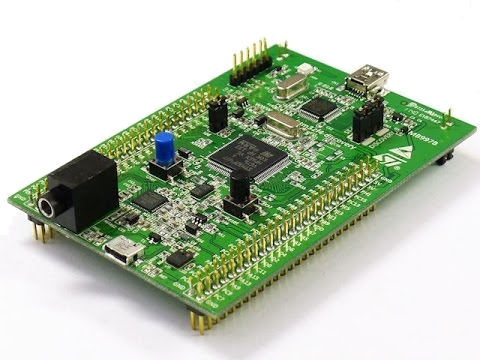
\includegraphics[width=5cm]{STM32F4_Discovery}
    \caption{Placa de desarrollo STM32F4 Discovery}
    \label{fig:STM32F4_Discovery}
\end{figure}

El \acrshort{MCU} cuenta con 3 buses SPI independientes que pueden funcionar en modo \textit{\gls{Full Duplex}}. El SPI$_1$  es capaz de funcionar hasta 42Mb/s mientras que los SPI$_2$ y SPI$_3$ pueden comunicar información hasta 21Mb/s. Los pines dedicados a dichos buses se pueden consultar en el \textit{Datasheet} del componente \cite{Datasheet_STM}.
\\Otra característica interesante de este \acrshort{MCU} es la presencia de forma nativa de un gestor de \acrshort{USB} \acrlong{OTG} (\acrshort{OTG}) permitiendo así conectar un dispositivo \acrshort{USB} para almacenar información a largo plazo.

\clearpage

\subsection{Alimentación\label{sec:Alimentación}}

Tras seleccionar todos los elementos se va a proceder a escoger una alimentación que permita a todos los dispositivos funcionar en condiciones óptimas.
\\La tabla \ref{tab:Alimentacion} muestra un resumen de todos los elementos presentes en el sistema junto con los rangos de voltaje recomendados por los fabricantes para su alimentación.

\begin{table} [h]
	\centering
	\begin{tabular}{|c|c|c|}
	\hline 
	Dispositivo & V$_{\text{min}}$ [V] & V$_{\text{max}}$ [V] \\ 
	\hline 
	Simblee BT & 1.8 & 3.6 \\ 
	\hline 
	ESP12-E & 3.0 & 3.6 \\ 
	\hline 
	STM & 1.8 & 3.6 \\ 
	\hline 
	ADS (Digital) & 1.8 & 3.6 \\ 
	\hline 
	ADS (Analógica) & 4.75 & 5.25 \\ 
	\hline 
	USB & 5 & 5 \\ 
	\hline 
	\end{tabular} 
	\caption{Rangos de alimentación de todos los elementos}
	\label{tab:Alimentacion}
\end{table}

De la tabla \ref{tab:Alimentacion} se deduce que para que todos los dispositivos funcionen correctamente \textbf{será necesario dotar a la placa de 5 voltios} con los que se podrá alimentar la parte analógica del ADS así como el USB mientras que la parte digital se puede alimentar en el rango de 3V a 3.6V. 

Por motivos de compatibilidad con el diseño anterior y tras comprobar que se cumple con los requisitos impuestos por los nuevos elementos del sistema se ha optado por mantener el mismo esquema de alimentación que en el proyecto base.

El sistema de alimentación se compone de dos partes principales, cada una encargada de proporcionar el voltaje deseado manteniendo el ruido generado por el mismo al mínimo.

\subsubsection{Alimentación 3.3V\label{sec:Alimentacion_3.3V}}
Para conseguir un voltaje de \textbf{3.3V} estable se ha utilizado el regulador \textbf{AZ1117C-3.3} ya que es capaz de conseguir una precisión para el voltaje de salida del $\pm$1\% así como un ruido de salida de 0.003\% V$_{\text{out}}$ entre 10Hz y 10kHz.
En la figura \ref{fig:Alim_3.3} se muestra el esquema eléctrico utilizado, que es una variación del circuito recomendado por el fabricante en su \textit{datasheet} \cite{Datasheet_3.3}.

\begin{figure} [h]
    \centering
    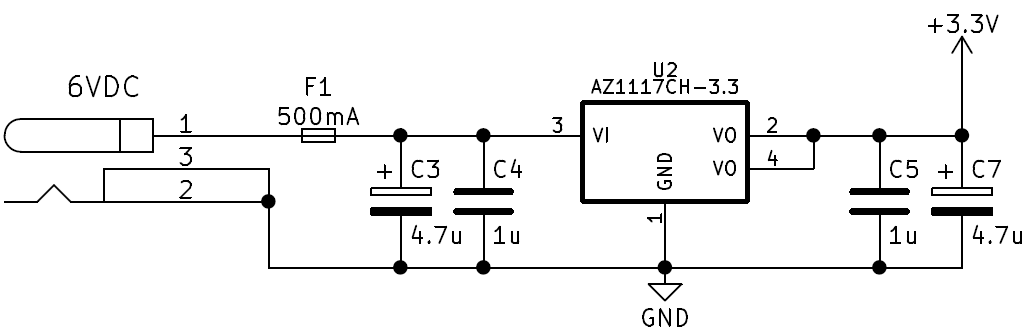
\includegraphics[width=10cm]{Alim_3_3}
    \caption{Esquema de alimentación a 3.3V}
    \label{fig:Alim_3.3}
\end{figure}

\subsubsection{Alimentación 5V\label{sec:Alimentacion_5V}}

Los 5V serán utilizados por el dispositivo de almacenamiento USB para su alimentación y por el ADS para generar los distintos voltajes de referencia que necesita para operar correctamente. Al afectar de forma directa a las mediciones realizadas por el ADS la eliminación de variaciones en este voltaje es crucial, pues estas supondrán un ruido añadido a la señal final.

El regulador encargado de proporcionar \textbf{5V} es el \textbf{MCP1711}. Este integrado está caracterizado por tener un rizado de salida menor al 1\% del voltaje de salida así como de poseer una corriente en reposo muy baja. Este último parámetro facilitará el diseño de un sistema portátil alimentado por baterías aumentando la duración de la misma. La figura \ref{fig:Alim_5} muestra el esquema eléctrico utilizado.

\begin{figure} [h]
    \centering
    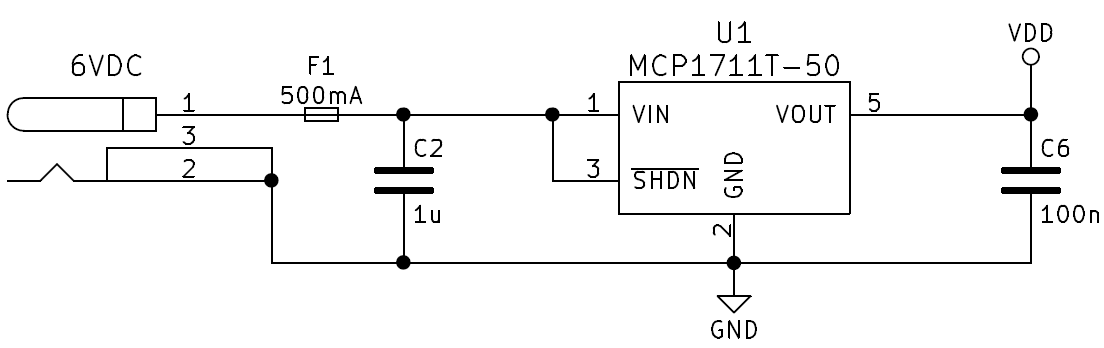
\includegraphics[width=10cm]{Alim_5}
    \caption{Esquema de alimentación a 5V}
    \label{fig:Alim_5}
\end{figure}

Para funcionar correctamente ambos integrados necesitan que el voltaje de entrada sea superior al voltaje de salida en un factor que en la documentación técnica recibe el nombre de ``\gls{Tension de Dropout}''(V$_{\text{DROP}}$).
\\De acuerdo al \textit{datasheet} de ambos reguladores, V$_{\text{DROP}}$ es para 3.3V y 5V, 1.3V y 0.43V respectivamente. Con esa información se deduce que el integrado que limita el diseño es el regulador de 5V de modo que con una entrada de al menos 5.43V ambos reguladores deberían funcionar correctamente.

Finalmente se ha optado por una \textbf{fuente de alimentación de 6V} ya que esto permitirá hacer uso de pilas o baterías para alimentar el sistema, dotándolo de independencia de la red eléctrica y eliminando el riesgo de electrocución.

\clearpage

\section{Circuito electrónico y esquemáticos\label{sec:Esquemáticos}}

El último paso de la fase de desarrollo será generar un \textbf{esquemático} capaz de englobar todos los elementos anteriormente presentados, interconectarlos y dar como resultado un sistema funcional.

En este punto es importante valorar dos alternativas de diseño, cada una con sus ventajas e inconvenientes: implementación de todo el circuito de cero o crear una placa que se conecte a la ya existente.

Si bien es cierto que para un diseño final crear una placa que englobe todos los componentes sería lo ideal, pues presentaría un formato más compacto y mejor presentación, hacerlo también supone crear una placa más grande y desaprovechar aquellas ya construidas en proyectos anteriores.

Teniendo en cuenta que se cuenta con varias tarjetas ya montadas y que el sistema está en fase de prototipo, se va a optar por la segunda opción, creando una \textbf{segunda tarjeta independiente} en la que se incluirán todos los elementos correspondientes a la gestión de las señales digitales del sistema, dejando las señales analógicas en la otra tarjeta. De esta forma la fase de diseño de la \acrshort{PCB} y de montaje se simplifica considerablemente y se \textbf{abaratan costes al reutilizarse componentes}.

Para la conexión con la otra tarjeta se aprovechará el espacio dejado por el módulo ESP12-E, pues para comunicarse con el ADS sólo es necesario el bus \acrshort{SPI} y todas las señales necesarias se encuentran accesibles desde los conectores de dicho módulo.

El sistema embebido en esta placa incluirá los elementos que se pueden ver en la figura \ref{fig:Esquematico_global}

\begin{figure} [h]
    \centering
    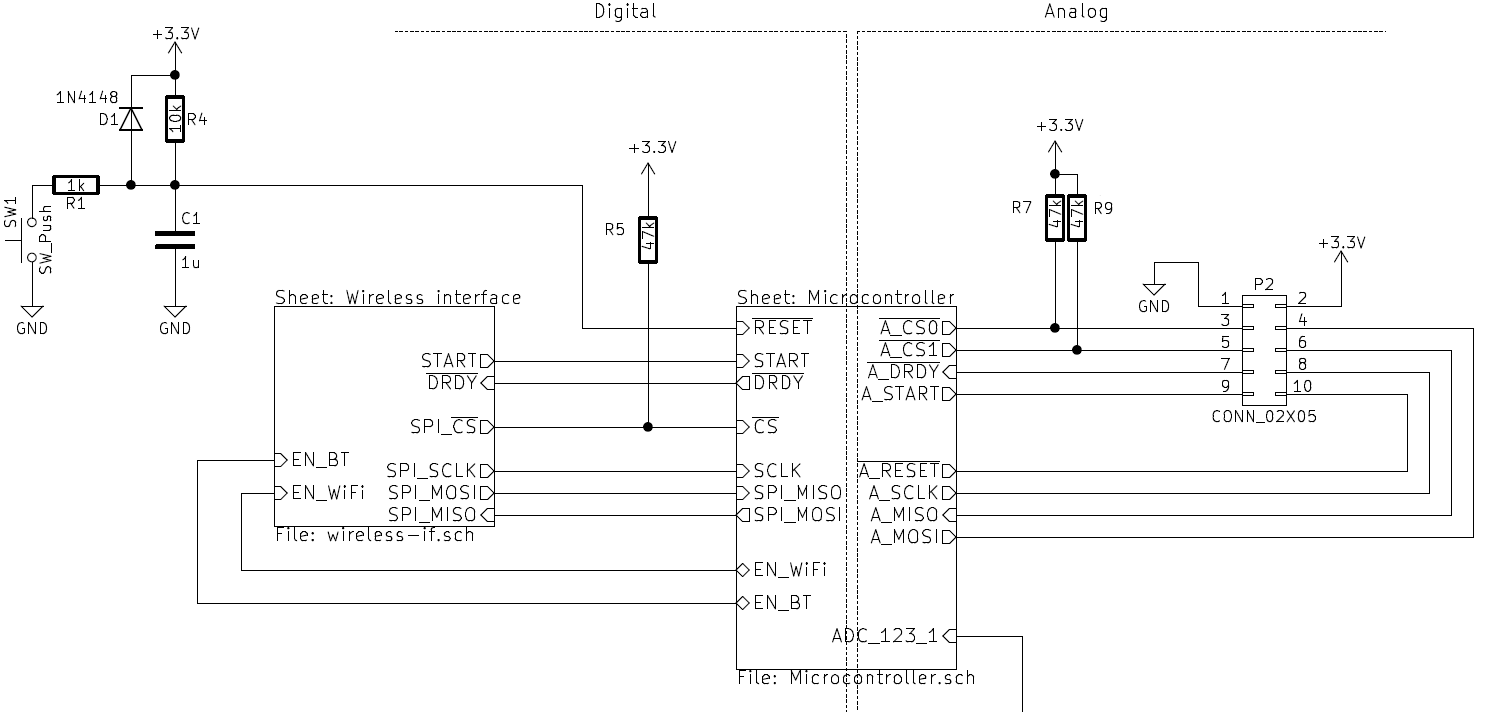
\includegraphics[width=14cm]{Esquematico_global}
    \caption{Esquema general del sistema}
    \label{fig:Esquematico_global}
\end{figure}

Se ha incluido en la placa un \textbf{botón de reinicio} con su correspondiente circuito electrónico así como una realimentación desde la alimentación hasta uno de los pines \acrshort{ADC} el microcontrolador para poder \textbf{monitorizar el estado de la batería}.

\subsection{Circuito de alimentación\label{sec:Esquemáticos_alim}}

Aunando los dos circuitos presentados en la sección \ref{sec:Alimentación} el resultado final es el obtenido en la figura \ref{fig:Alim_final}.

\begin{figure} [h]
    \centering
    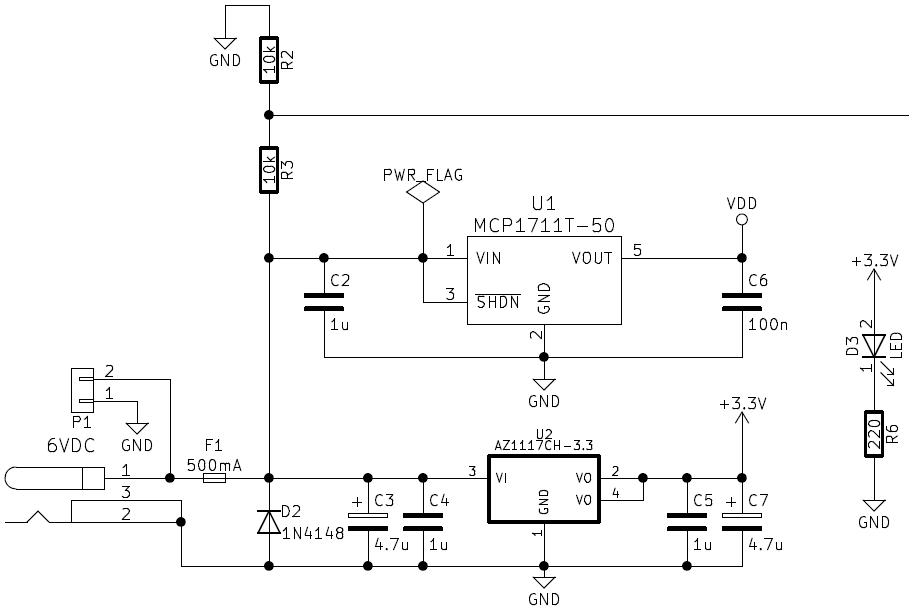
\includegraphics[width=14cm]{Alim_final}
    \caption{Esquemático final del circuito de alimentación}
    \label{fig:Alim_final}
\end{figure}

El \textbf{fusible} (F1) garantiza que la máxima corriente que consumirá el dispositivo es de 500mA, \textbf{evitando} así que el sistema o el paciente sufran \textbf{daños} en caso de un cortocircuito. Adicionalmente se ha incluido un diodo \acrshort{LED} cuya función es indicar el estado de la placa. Si la placa ha encendido correctamente o si se encuentra en funcionamiento el \acrshort{LED} se encenderá.

El diodo (D2) junto con el condensador (C3) evitarán que los transitorios afecten al voltaje de entrada asegurando así que la alimentación que recibirán ambos integrados será lo más estable posible.

Con el objetivo de \textbf{monitorizar el estado de la batería} se ha utilizado el \textbf{\acrshort{ADC} incorporado en el propio microcontrolador}. Como la señal de entrada se encuentra fuera del rango soportado en las especificaciones del STM se ha optado por incorporar las resistencias R2 y R3 formando un divisor de tensión utilizando así la señal resultante para realizar las medidas.

\clearpage

\subsection{Microcontrolador\label{sec:Esquemáticos_micro}}

El \textbf{microcontrolador es el núcleo del sistema}. Este hace de \textbf{centro de control} de todas las señales digitales que se transmiten así como de \textbf{gestor de dispositivos}, decidiendo que dispositivos se encuentran activos en cada momento. 
Para gestionar que dispositivos se encuentran habilitados se ha sustituido el \textit{jumper} de la placa original por \acrshort{GPIO} del microcontrolador. De esta forma se consigue mayor flexibilidad, automatización y se optimiza el consumo. 

Adicionalmente se ha integrado un \acrshort{LED} conectado al pin PA9 que dotará a la placa de indicadores visuales del estado en el que se encuentra.

La figura \ref{fig:Esquematico_micro} muestra una representación del integrado junto con todos los elementos con los que está conectado.

\begin{figure} [h]
    \centering
    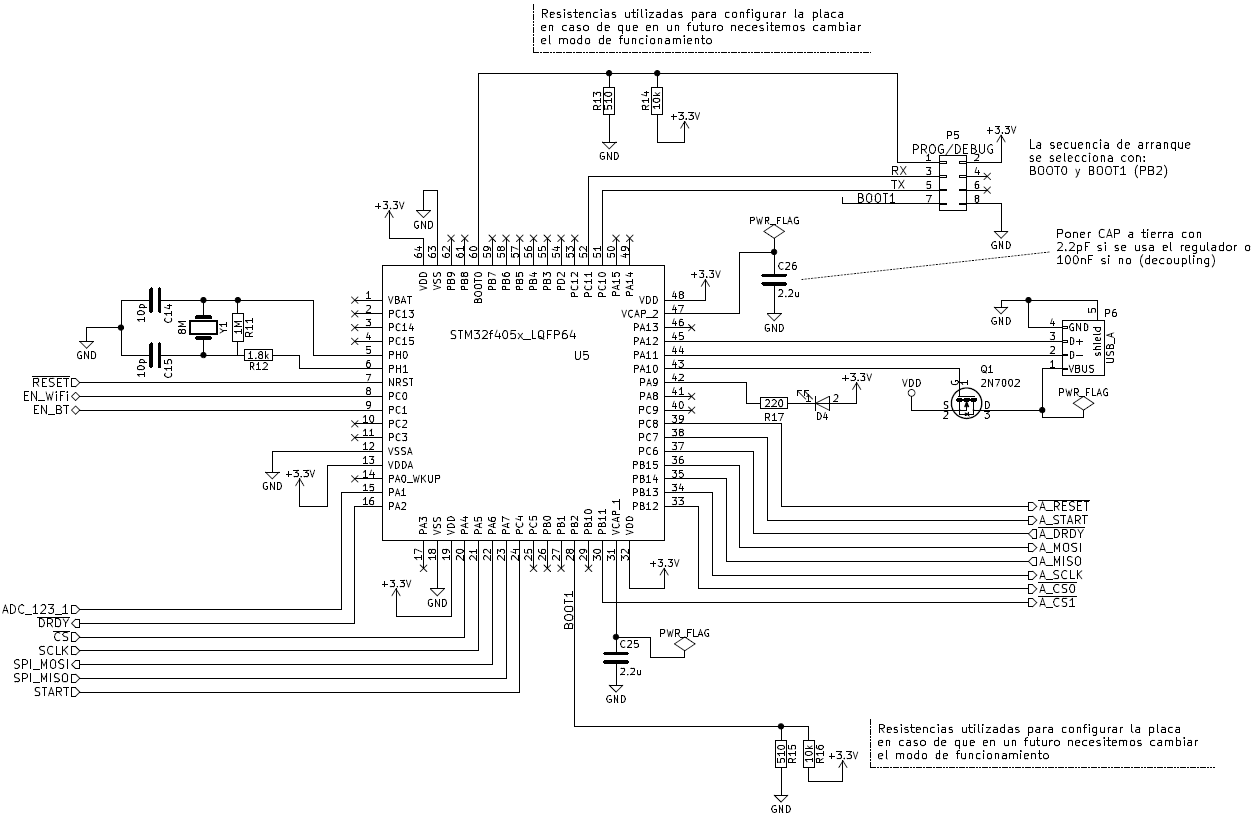
\includegraphics[width=\textwidth]{Esquematico_micro}
    \caption{Esquemático del microcontrolador}
    \label{fig:Esquematico_micro}
\end{figure}

El \textbf{modo de arranque} del dispositivo viene determinado por el estado de los pines Boot0 y Boot1. Haciendo uso de las resistencias R13, R14, R15 y R16 se consigue forzar que en condiciones normales de operación el STM \textbf{arranque desde la memoria Flash integrada}. 
\\Con el objetivo de \textbf{reprogramar el microcontrolador} se ha añadido el conector P5. Dicho conector permite alternar entre los distintos modos de arranque del STM e interactuar con el por UART. Esta última característica será la que permitirá subir el código a ejecutar pero también brinda funciones de \textit{debug}.

\clearpage

El sistema aprovecha dos de los tres buses \acrshort{SPI}. El bus SPI1, capaz de transmitir a 41Mb/s, se ha reservado para la comunicación ESP12-E $\Longleftrightarrow$ STM32F4 mientras que el utilizado para comunicarse con los ADS es el SPI2, con una velocidad de hasta 21Mb/s.

Aunque el \acrshort{MCU} puede trabajar con un oscilador interno, se ha optado por la utilización de un \textbf{oscilador externo basado en un cristal de cuarzo}. Esa opción permite una mayor precisión en el reloj y la posibilidad de usar \acrshort{PLL} para aumentar la frecuencia de trabajo del procesador.
\\El circuito asociado al cristal se puede observar en la parte superior izquierda de la figura \ref{fig:Esquematico_micro} pero se incluye a continuación para facilitar la lectura de este documento:

\begin{figure} [h]
    \centering
    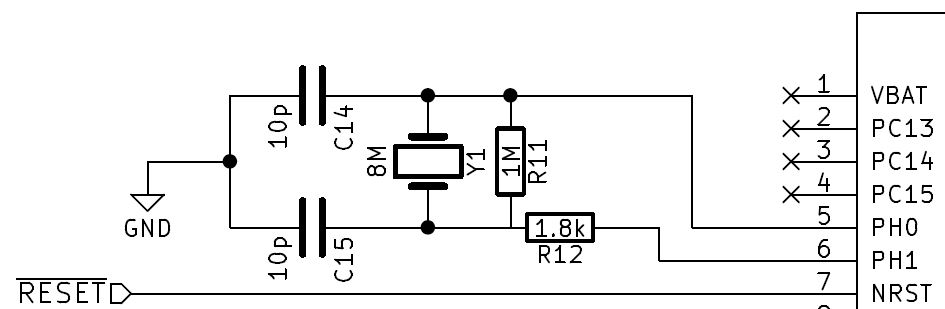
\includegraphics[width=10cm]{Detalle_cristal}
    \caption{Detalle del circuito asociado al oscilador externo}
    \label{fig:Detalle_cristal}
\end{figure}


Para realizar un diseño óptimo del circuito del oscilador se ha utilizado como orientación la hoja de características del dispositivo junto con una guía de buenas prácticas \cite{Guia_Oscilador}, ambos proporcionados por el fabricante. La configuración utilizada a nivel de software para la gestión de dicho reloj se explicará en mayor profundidad en el capítulo \ref{sec:Implementacion_soft}.

Se han añadido todos los condensadores recomendados por el fabricante. Algunos deben tener una capacidad determinada en función del modo de funcionamiento del microcontrolador (C25 y C26), otros, denominados \textbf{condensadores de desacoplo}, tienen como objetivo eliminar el ruido de altas frecuencias de la zona de alimentación. Un condensador a resaltar es el C11, denominado \textbf{\textit{Bulk}} y su función es garantizar una alimentación lo más estable posible.

\begin{figure} [h]
    \centering
    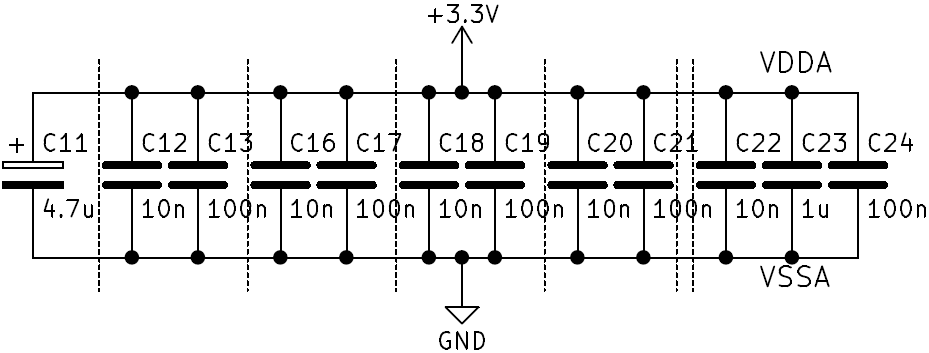
\includegraphics[width=10cm]{Condensadores_micro}
    \caption{Condensadores Bulk (C11) y de desacoplo}
    \label{fig:Condensadores_micro}
\end{figure}

 Por simplicidad y legibilidad se han agrupado todos los condensadores en una zona del esquemático, pero a la hora de diseñar la PCB será necesario tener presente que para que el dispositivo funcione correctamente estos últimos \textbf{deben localizarse lo más cerca posible de los pines de alimentación}.

Finalmente, como el \acrshort{MCU} tiene la capacidad de interactuar directamente con dispositivos \acrshort{USB}, con el objetivo de implementar en un futuro características que aprovechen dicha capacidad se ha añadido un conector \acrshort{USB} cuyo bus de alimentación se encuentra controlado por el propio \acrshort{MCU}. De esta forma es posible habilitar y deshabilitar el dispositivo USB y reducir el consumo.

\subsection{Interfaz inalámbrica\label{sec:Esquematico_inalambrica}}

Para finalizar con la parte del diseño, se incluirá una explicación de los esquemáticos necesarios para hacer funcionar los dos microcontroladores encargados de transmitir la información a través de Wifi y Bluetooth.

\subsubsection{ESP12-E\label{sec:Esquematico_ESP}}

El ESP necesita, al igual que el STM, condensadores Bulk y de desacoplo. Ambos se pueden apreciar en la figura \ref{fig:Esquematico_ESP} en la parte inferior izquierda y deberán estar localizados en la \acrshort{PCB} lo más cerca posible de los pines de alimentación.

\begin{figure} [h]
    \centering
    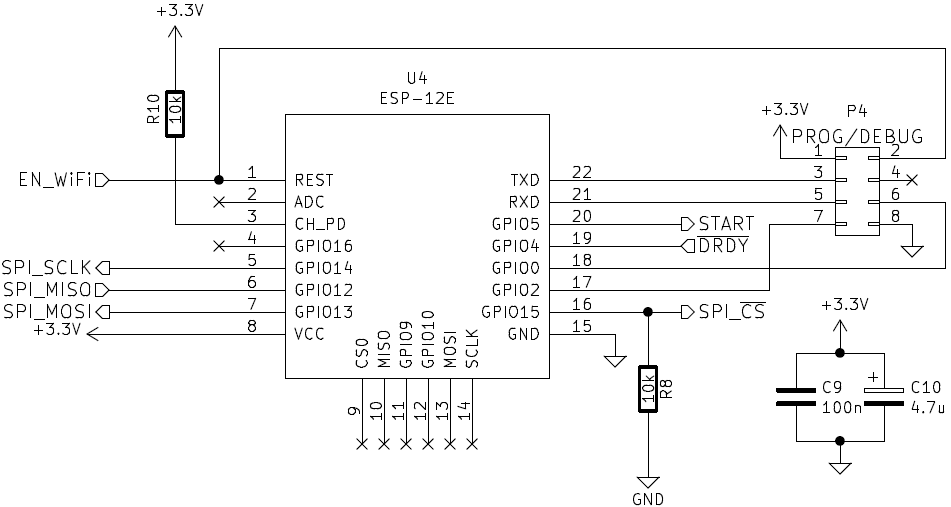
\includegraphics[width=\textwidth]{Esquematico_ESP}
    \caption{Esquemático del ESP-12E}
    \label{fig:Esquematico_ESP}
\end{figure}

La resistencia R10 fuerza al ESP a estar en un estado activo salvo que el STM (Máster del sistema) lo deshabilite haciendo uso del pin ``EN\_WIFI''. 
\\El modo de arranque del ESP viene definido por la resistencia R8 junto con el conector P4. Para poder ponerlo en modo programación sólo será necesario cortocircuitar los pines 6 y 8. El acceso al bus UART se realizará a través de los pines 3 y 5.

\subsubsection{Bluetooth Simblee\label{sec:Esquematico_BT}}

Para el dispositivo Bluetooth se ha incluido otro conector de programación. En esta ocasión sólo serán necesarios los pines 2, 3 y 4 para la programación ya que el \acrshort{IDE} de Arduino se encargará de la gestión de los diferentes modos de arranque el dispositivo.

\begin{figure} [h]
    \centering
    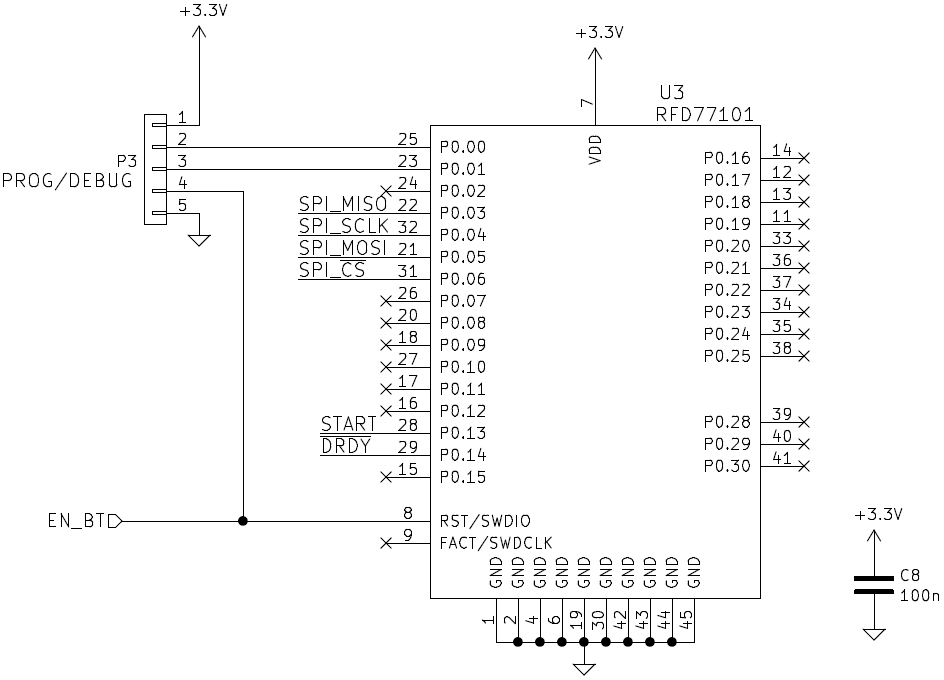
\includegraphics[width=14cm]{Esquematico_BT}
    \caption{Esquemático del dispositivo Bluetooth Simblee}
    \label{fig:Esquematico_BT}
\end{figure}

El bus \acrshort{SPI} así como los de DRDY y START han sido conectados al STM ya que dichas conexiones serán necesarias para la transmisión de datos entre el STM y el módulo Bluetooth.

En esta ocasión se ha dejado sólo un condensador de desacoplo dado que los de \textit{Bulk} dispuestos para los otros dispositivos suplen la necesidad de utilizar otro para este.

Todos los esquemáticos presentados a lo largo de este capítulo han sido generados haciendo uso de la herramienta KiCad. Al ser un esquemático, su lectura e interpretación es independiente de la herramienta siendo el elemento ``PWR\_FLAG'' (presente en algunas figuras) el único exclusivo de dicha herramienta. Este elemento sive para evitar errores, ya que todos los pines categorizados como pines de alimentación que no lleven un ``PWR\_FLAG'' provocarán una alerta al compilar y generar el esquemático. 